\documentclass[]{IEEEtran}
% some very useful LaTeX packages include:
%\usepackage{cite}      
\usepackage{graphicx}   
\usepackage{subfigure} 
\usepackage{url}       
\usepackage{amsmath}    
\usepackage{caption2}
% Your document starts here!
\begin{document}

% Define document title and author
	\title{Weekly Report}
	\author{Adviser: Prof. Yang Wen \\Student: Cheng Wensheng\\ Period: 2018.7.22-7.29
	}
	\markboth{Visual Information Processing Group}{}
	\maketitle

% Write abstract here
\begin{abstract}
	This week I mainly put my effort on writing the government proposal and revising software.
\end{abstract}

% Each section begins with a \section{title} command
\section{Writing proposal}
	% \PARstart{}{} creates a tall first letter for this first paragraph
	\PARstart{T}{here} is a government project about environmental management, and we need to write the proposal in this week. 
	\begin{itemize}
		\item My work is the part of river management system and engineering implementation plan. 
		\item At first, I wrote about river supervisor system, which means to divide the whole river into parts, and appoint someone to be in charge of this part. Then after teachers talking about the draft, I changed the river supervisor system into grid based management system, which is more comprehensive.
		\item Finally, I wrote about 30 pages and revised it according to the requirement of the director.
		
		Fig.~\ref{fig:mp} is the system function pipeline. Fig.~\ref{fig:ss} is the system architecture.
	\end{itemize}

% Main Part
\section{Revising software}
	% LaTeX takes complete care of your document layout.
	We uploaded our software last week, and the feedback shows that we need to revise our software.
	\begin{itemize}
		\item The output name is required to be the same with the input image, so is the output name in the XML file. 
		\item The ouput image format needs to be consisted with input image. They are both in bmp format.		
		\item We uploaded software again, and got the results. I need to try more methods to improve precision. 
	\end{itemize}
\newpage
\begin{figure}[!hbt]
%		 Center the figure.
		\vspace{0.3cm}
%		\hspace{50cm}
		\begin{center}
			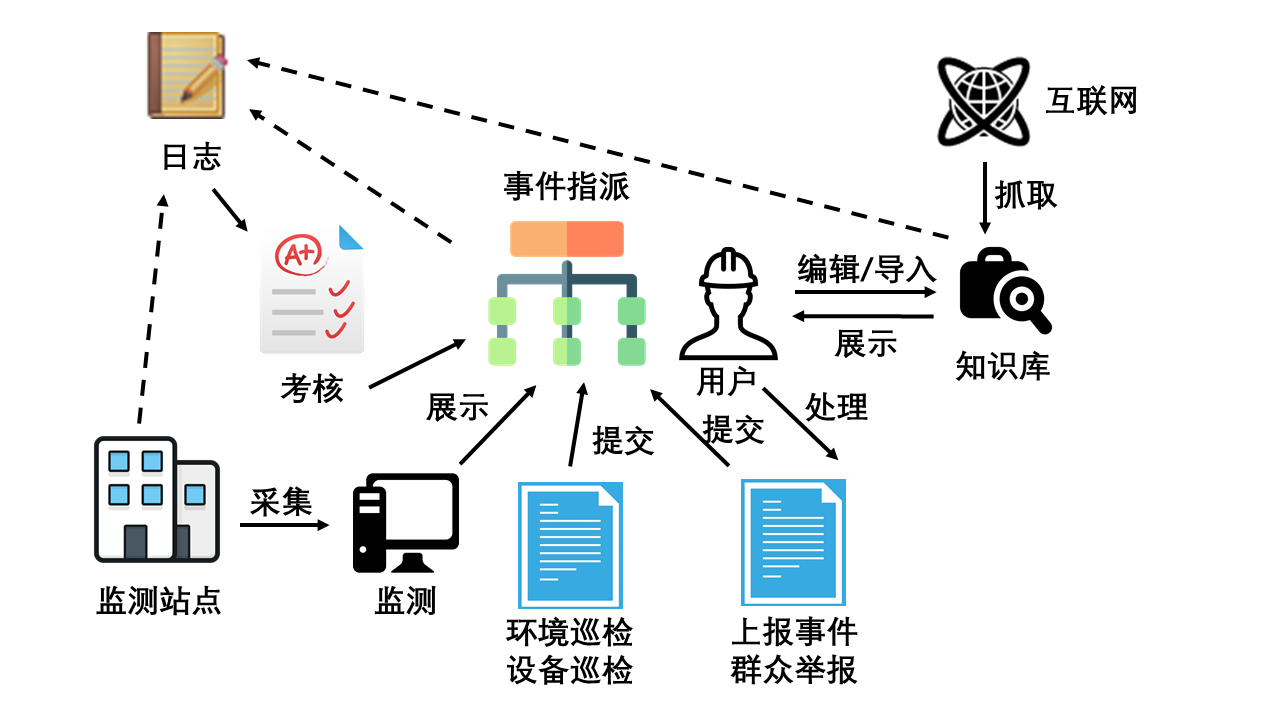
\includegraphics[width=0.9\columnwidth]{gt}
				%		 Create a subtitle for the figure.
			\caption{System function}
			\label{fig:mp}
		   % \vspace{0.2cm}
			
\includegraphics[width=0.9\columnwidth]{pred}
				%Create a subtitle for the figure.
			\caption{System architecture}
			\label{fig:ss}
		\end{center}
	\end{figure}

% Your document ends here!
\end{document}